\documentclass{beamer}
\usepackage[latin1]{inputenc}
\usetheme{boxes}
\title[Regexes in Python]{Regular Expressions in Python Tutorial}
\author{Michelle Fullwood}
\date{PyLadies Meetup Aug 2013}
\usepackage{color}
\newsavebox{\mysavebox}
\usepackage{listings}

\usepackage{verbdef}

\definecolor{mygreen}{rgb}{0,0.6,0}
\definecolor{mygray}{rgb}{0.5,0.5,0.5}
\definecolor{mymauve}{rgb}{0.58,0,0.82}

\lstset{ %
  backgroundcolor=\color{white},   % choose the background color; you must add \usepackage{color} or \usepackage{xcolor}
  basicstyle=\ttfamily\footnotesize,        % the size of the fonts that are used for the code
  keywordstyle=\bfseries,
  identifierstyle=\color{red},     % object names
  commentstyle=\rmfamily\itshape, % italic comments
  stringstyle=\slshape,           % strings
  breakatwhitespace=false,         % sets if automatic breaks should only happen at whitespace
  breaklines=true,                 % sets automatic line breaking
  captionpos=b,                    % sets the caption-position to bottom
  commentstyle=\color{mygreen},    % comment style
  deletekeywords={...},            % if you want to delete keywords from the given language
  escapeinside={\%*}{*)},          % if you want to add LaTeX within your code
  extendedchars=true,              % lets you use non-ASCII characters; for 8-bits encodings only, does not work with UTF-8
  frame=single,                    % adds a frame around the code
  keepspaces=true,                 % keeps spaces in text, useful for keeping indentation of code (possibly needs columns=flexible)
  keywordstyle=\color{blue},       % keyword style
  language=Python,                 % the language of the code
  morekeywords={*,^,...},            % if you want to add more keywords to the set
  numbers=none,                    % where to put the line-numbers; possible values are (none, left, right)
  numbersep=5pt,                   % how far the line-numbers are from the code
  numberstyle=\tiny\color{mygray}, % the style that is used for the line-numbers
  rulecolor=\color{black},         % if not set, the frame-color may be changed on line-breaks within not-black text (e.g. comments (green here))
  showspaces=false,                % show spaces everywhere adding particular underscores; it overrides 'showstringspaces'
  showstringspaces=false,          % underline spaces within strings only
  showtabs=false,                  % show tabs within strings adding particular underscores
  stepnumber=2,                    % the step between two line-numbers. If it's 1, each line will be numbered
  stringstyle=\color{mymauve},     % string literal style
  tabsize=2,                       % sets default tabsize to 2 spaces
%  title=\lstname                   % show the filename of files included with \lstinputlisting; also try caption instead of title
}



\begin{document}

\begin{frame}
\titlepage
\end{frame}


\begin{lrbox}{\mysavebox}
\begin{lstlisting}
PCOD   QTY   DEPT    COST
A169   100   Micro   0.58
PDA1   1     Xray    600.00
X280   5     ER      199.99
...
\end{lstlisting}
\end{lrbox}

\begin{frame}{Motivating regular expressions}

{\bf Scenario:} You're evaluating Acme Company's products for a hospital.
You're given a text file containing purchase records from Acme.
Looking through the text file, however, you see that purchases from other companies
are included as well, with no mention of which ones come from which!

\vspace{1.5em}
{\usebox{\mysavebox}}
\vspace{1em}

Luckily, you know that Acme's product codes consist of one
uppercase letter followed by three digits.

\end{frame}


\begin{frame}{Motivating regular expressions}

So you get to work with a script:

\lstinputlisting[language=Python]{code_for_slides/slide2.py}

It's a bit clunky, but it works.

\end{frame}

\begin{lrbox}{\mysavebox}
\begin{lstlisting}
'...The X701 vacuum cleaner really sucked!...'
'...The gloves(P180) felt sticky...'
\end{lstlisting}
\end{lrbox}

\begin{frame}{Motivating regular expressions}

The next step in your evaluation is to collate comments
emailed to you by hospital staff. These were free text,
so you need to extract the product codes from within them
to know which evaluation refers to which product.

\vspace{1.5em}
{\usebox{\mysavebox}}
\vspace{1em}

You might be able to think of ways to program this,
but really...

\begin{center}
\textcolor{red}{It's time to bust out regular expressions.}
\end{center}

\end{frame}

\begin{frame}{Motivating regular expressions}

What we want is a way to simply search for ``one uppercase letter
followed by three digits''. We can do this using (1) a regular
expression and (2) the \lstinline$search$ function provided
by Python's \lstinline$re$ module:

\vspace{1em}
\lstinputlisting[language=Python]{code_for_slides/slide4.py}

\end{frame}

\begin{frame}{Just what are regular expressions, anyway?}

Regular expressions are strings that describe other sets of strings.

\begin{center}
\begin{tabular}{cc}
\lstinline$`[A-Z]$ & \lstinline$\\d\{3\}'$  \\
$\left\{\begin{matrix} A \\ B \\ ... \\ Z \end{matrix}\right\}$ &
$\left\{\begin{matrix} 0 \\ 1 \\ ... \\ 9 \end{matrix}\right\} x 3$ \\
\end{tabular}
\end{center}

What we need to know to write regular expressions:
\begin{itemize}
 \item How to define sets of characters
 \begin{itemize}
   \item Metacharacters  \lstinline$\\w, \\s, \\d$ 
   \item Character sets  \lstinline$[A-Z], [AGCT], [^AGCT]$
 \end{itemize}
 \item How to define how many times to repeat them
 \begin{itemize}
   \item A specific number of times \lstinline$\{3,5\}, ?$
   \item An unlimited number of times \lstinline$*,+$
 \end{itemize}
\end{itemize}

\end{frame}

\begin{frame}{Plan for today}

We'll learn:
\begin{itemize}
 \item The pattern language for regular expressions
 \item The Python \lstinline$re$ functions that allow us to work with regexes
\end{itemize}

\end{frame}

\begin{frame}{Playing along}

How to practise the code as we go along:
\begin{itemize}
 \item Install \lstinline$git$ (if you attended last month's meeting, you already have it!)
 \item From the command line: \lstinline$git clone https://github.com/michelleful/RegexTutorial.git$
 \item Run the exercises from the command line interface:
 \begin{itemize}
   \item \lstinline$cd exercises$
   \item Open up \lstinline$ex1.py$ etc as we move along
   \item Edit and run \lstinline$python ex1.py$ from the CLI
 \end{itemize}
 \item OR if you have iPython:
   \begin{itemize}
    \item Run \lstinline$ipython notebook$ from the command line
    \item A browser window will automatically open
    \item Select the only notebook, follow the instructions therein
   \end{itemize}
 \item OR if you don't have \lstinline$git$, play with the regexes online
   \begin{itemize}
    \item Enter regexes and strings into \lstinline$http://www.pythonregex.com/$
   \end{itemize}
\end{itemize}

\end{frame}

\begin{frame}{Aside: why r''?}

All the regular expressions you'll see today will be within \lstinline$r''$.
What's the deal with the \lstinline$r$?

\bigskip

\lstinline$r$ stands for raw strings. It means that backslashes are interpreted
as backslashes, as opposed to regular strings, where they're interpreted as
special characters.

\bigskip

You could define regexes using regular Python strings, but then you'd need
to escape every backslash.

\begin{center}
\lstinline$r'\\d{3}' == '\\\\d{3}'$
\end{center}

And if you're searching for backslashes, that would mean needing to write:
\lstinline$'\\\\\\\\'$, as opposed to just \lstinline$r'\\\\'$.

\end{frame}

\begin{frame}{Metacharacters}

Metacharacters are pre-defined sets of characters.
 \begin{itemize}
  \item \lstinline$.$ matches ANY character except the newline character \lstinline$\\n$*
  \item \lstinline$\\d$ matches digits 0 through 9
  \item \lstinline$\\w$ matches alphanumeric characters and underscore \_
  \item \lstinline$\\s$ matches whitespace characters
    \begin{itemize}
     \item Spaces 
     \item Tabs \lstinline$\\t$
     \item Newlines \lstinline$\\n\\r$
    \end{itemize}
 \end{itemize}

 \bigskip
 $\rightarrow$ Exercise 1
\end{frame}

\begin{frame}{Defining sets of characters}
 \begin{itemize}
  \item List characters individually
    \begin{itemize}
      \item \lstinline$[AGCT]$ matches one character A, G, C or T.
      \item \lstinline$[\\s\\d]$ matches one whitespace character or digit
    \end{itemize}
  \item Define a range of characters
    \begin{itemize}
      \item \lstinline$[A-T]$ matches one character between A and T.
      \item \lstinline$[1-7]$ matches one digit between 1 and 7.
      \item Ranges as defined by ASCII or Unicode tables
      \item You can combine ranges: \lstinline$[a-cA-C]$
    \end{itemize}
 \end{itemize}

 \bigskip
 $\rightarrow$ Exercise 2

\end{frame}

\begin{frame}{Defining where a regular expression applies}

We can say a regex has to be at the start or the end of the string, or at word boundaries,
with more special characters.

\begin{itemize}
 \item \lstinline$^$ -- beginning of line
 \item \lstinline$\$$ -- end of line 
 \item \lstinline$\\b$ -- word boundary
\end{itemize}

Examples: $\rightarrow$ Exercise 3
\begin{itemize}
 \item \lstinline$^Hallo\$$
 \item \lstinline$\\bHallo\\b$
\end{itemize}

\end{frame}

\verbdef{\specialchartext}{\^ \$ \. \\}

\begin{frame}{Escaping characters}

$\rightarrow$ Exercise 4

\bigskip

Why didn't the regex(es) work? (Discuss.)

\begin{itemize}
 \item When using characters that also have a special meaning, we have to escape them with a backslash
 \item \specialchartext
 \item Exception: within character sets [], metacharacters have their regular meaning, except backslashes.*
\end{itemize}

\end{frame}

\begin{frame}{Defining complements of a set}

Sometimes it's easier to define a set of characters as ``everything other than X''.

\begin{itemize}
  \item \lstinline$\\S$ -- all non-whitespace characters
  \item \lstinline$\\W$ -- all non-alphanumeric characters (also excludes underscore)
  \item \lstinline$\\D$ -- all non-numeric characters
  \item \lstinline$[^A-D]$ -- all characters other than A, B, C, D
\end{itemize}

\bigskip
$\rightarrow$ Exercise 5

\end{frame}

\begin{frame}{Repeating things}

So far, whenever we've wanted to match, say, three digits, we've just been writing
\lstinline$\\d\\d\\d$. This could easily get old if we want to match thirty or a thousand digits.
It gets impossible when we want to match any arbitrary number of digits.
Fortunately, regular expressions let us express this very succinctly.

\end{frame}

\begin{frame}{Repeating things}

\begin{itemize}
 \item \lstinline$*$ means 0 or more times
 \item \lstinline$+$ means 1 or more times
 \item \lstinline$?$ means 0 or 1 times
 \item \lstinline$\{n\}$ means n times exactly
 \item \lstinline$\{m,\}$ means m or more times
 \item \lstinline$\{m,n\}$ means m--n times
 \item Example: \lstinline$.*$ matches anything
 \item Example: \lstinline$[a-c]\{3\}$ matches 'abc' etc
\end{itemize}

\bigskip
$\rightarrow$ Exercise 6

\end{frame}

\begin{frame}{Specifying alternatives}

Sometimes you want to say match this OR that.
You can do that with the \lstinline$|$ operator.

\begin{itemize}
  \item \lstinline$Alex|Bill|Conrad$ matches any of these three names
\end{itemize}

Sometimes there can be confusion about what \lstinline$|$ refers to.
In such cases, put brackets around the alternatives.

\begin{itemize}
  \item \lstinline$Jim and (Alex|Bill|Conrad)$ matches 'Jim and Alex', 'Jim and Bill', etc
\end{itemize}

\bigskip
$\rightarrow$ Exercise 7

\end{frame}

\begin{frame}{Taking a step back}

We've gone through a lot of the syntax for regular expressions.

\begin{enumerate}
  \item Any questions?
  \item Any challenging patterns you'd like to try as a group to express as a regex?
\end{enumerate}
\end{frame}

\begin{frame}{Python functions for dealing with regular expressions}

\begin{itemize}
  \item \lstinline$re.find(regex, string)$ -- returns a match group if the string starts with the regex pattern, \lstinline$None$ otherwise.
  \item \lstinline$re.search(regex, string)$ -- returns a match group if the string contains the regex pattern, \lstinline$None$ otherwise.
\end{itemize}

\bigskip
$\rightarrow$ Exercise 8

\end{frame}

\begin{frame}{Doing stuff with regular expressions}

So far we've just been checking for matches with regexes. But we can do more!

\bigskip

We can:
\begin{itemize}
 \item Capture the matches and do stuff with them
 \item Replace the match with something else
 \item Split a string whenever you match the regex \\ (not covered today)
\end{itemize}

\end{frame}

\begin{frame}{Capturing matches}

We capture matches by putting brackets around the part we want to extract.
Then access the matched bits via the match object returned by \lstinline$re.find()$ and \lstinline$re.search()$

\bigskip

Example: We want to match strings that look like a first name followed by a last name,
and extract them separately.

\lstinputlisting[language=Python]{code_for_slides/name_match.py}

$\rightarrow$ Exercise 9

\end{frame}

\begin{frame}{Capturing multiple matches}

Notice on the previous slide that we only captured the first instance of each name.
In order to capture multiple matches, use \lstinline$re.findall()$.

\lstinputlisting[language=Python]{code_for_slides/find_all.py}

$\rightarrow$ Exercise 10

\end{frame}

\begin{frame}{Nesting capturing parentheses}

You can actually nest capturing parentheses. For instance, if we put
another set of parentheses around the example in the preceding slide, 
we get this:

\bigskip

\lstinputlisting[language=Python]{code_for_slides/find_all_nested.py}

\end{frame}


\begin{frame}{Non-greedy matching}

By default, operators like * and + are ``greedy''. They match as much
as they can. In order to make it match in a ``non-greedy'' way, add a ?
after the operator.

\lstinputlisting[language=Python]{code_for_slides/greediness.py}

\end{frame}

\begin{frame}{Non-capturing parentheses}

$\rightarrow$ Exercise 11

\bigskip

Earlier, we used parentheses  \lstinline$()$ to disambiguate what the \lstinline$|$ operator
referred to. But now we're getting unwanted captures.

\bigskip

The solution here is to use non-capturing parentheses. Replace the regular 
parentheses  \lstinline$(...)$ with  \lstinline$(?P:...)$ whenever you
need to use parentheses but don't want to capture the result.

\end{frame}

\begin{frame}{Replacing matches}

Here's another thing you can do with regexes -- replace some matched segment
with another. For example, you're writing a novel with the protagonist Edward,
who has various nicknames. Halfway through you decide to rename him just Paul.

\lstinputlisting[language=Python]{code_for_slides/sub_example.py}

(This is a bit of a stupid example because you could just use string replacement,
but it's a first step.)

\bigskip

$\rightarrow$ Exercise 12

\end{frame} 

\begin{frame}{Back references}

Suppose you want to protect all the email addresses
on your site from being slurped up by a robot. You
want to replace '@' with ' (at) ', but only in valid email
addresses and not, say, Twitter handles.

\bigskip

We want to reuse our reliable ol' regex: \lstinline$r'\w+@\w+\\.(?:com|org|edu|net)'$

\bigskip

Problem: how do we replace the @ sign while leaving the stuff
on either side intact? We can do this by capturing what's to the left and right using parentheses,
then reproducing them in our replace string with {\bf back references}.

\end{frame}

\begin{frame}{Back references}

Backreferences are referred to with \lstinline$\\n$. \lstinline$\\1$
refers to the first match, \lstinline$\\2$ to the second match, etc.

\lstinputlisting[language=Python]{code_for_slides/backrefs.py}

\bigskip

$\rightarrow$ Exercise 13

\end{frame}

\begin{frame}{Back references}

You can also use back references within the regex you use to match
to find multiple copies of the same string.

\lstinputlisting[language=Python]{code_for_slides/backrefs2.py}

\bigskip

\end{frame}

\begin{frame}{Advanced topics}

\begin{itemize}
 \item Compiling regular expressions
 \item Flags
 \item Named matches
\end{itemize}

\end{frame}

\begin{frame}{Compiling regular expressions}

Sometimes you might see code like this:

\lstinputlisting[language=Python]{code_for_slides/compiled_regex.py}

{\small Once you have compiled your regex, you can call all the \lstinline$re$ functions
directly as methods of the compiled regex. }

\bigskip

{\small Compiling your regex is a good idea but not necessary for small
programs because Python will compile and cache your last few regexes anyway.}

\end{frame}

\begin{frame}{Flags}

Flags change the way metacharacters, character sets and spaces are interpreted.

\bigskip

Some of the flags:
\begin{itemize}
  \item \lstinline$re.IGNORECASE$ or \lstinline$re.I$ -- case-insensitive matching
  \item \lstinline$re.MULTILINE$ or \lstinline$re.M$ -- makes \lstinline$^$ and \lstinline$\$$ match beginning and end of each newline
  \item \lstinline$re.DOTALL$ or \lstinline$re.S$ -- makes . match any character {\it including} \lstinline$\\n$
  \item \lstinline$re.UNICODE$ or \lstinline$re.U$ -- \lstinline$\\w,\\b$ reinterpreted according to Unicode definition
  \item \lstinline$re.VERBOSE$ or \lstinline$re.V$ -- ignores whitespace and lets you use comments within the regex
\end{itemize}

\end{frame}

\begin{frame}{Flags}

How to set flags:

\bigskip

On any \lstinline$re$ function, add the flags as the last parameter:

\begin{itemize}
  \item \lstinline$re.search(myregex, mystring, re.U)$
  \item \lstinline$re.compile(myregex, re.MULTILINE | re.DOTALL)$
\end{itemize}

\end{frame}

\begin{frame}{Named matches}

It's possible to identify groups by names:

\lstinputlisting[language=Python]{code_for_slides/named_matches.py}

This can be helpful for keeping track of multiple matches.

\end{frame}

  
\begin{frame}{A word of caution on your newfound power...}

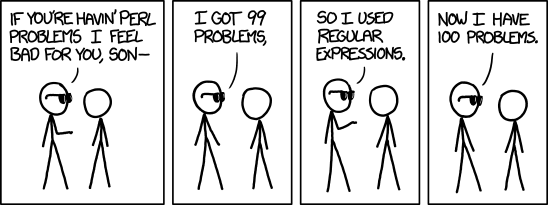
\includegraphics[scale=0.5]{images/perl_problems.png} 

http://xkcd.com/1171/

\end{frame}

\begin{frame}{When not to use regular expressions}

Regular expressions are powerful, but you shouldn't reach for them whenever you need some string matching.

\bigskip

In particular, don't use regular expressions when:
\begin{itemize}
 \item A simple string operation will do
	\begin{itemize} 
      \item \lstinline$'abc' in mystring$
      \item \lstinline$mystring.replace('x','y')$
    \end{itemize}
 \item You're parsing something that uses matching brackets, e.g. HTML and XML.
   \begin{itemize}
     \item Use the \lstinline$BeautifulSoup$ or \lstinline$lxml$ libraries instead!
   \end{itemize}
\end{itemize}

\end{frame}

\begin{frame}{The end}

That's all I have to teach you about regular expressions.

\bigskip

Now get out there and be a hero.

\begin{center}
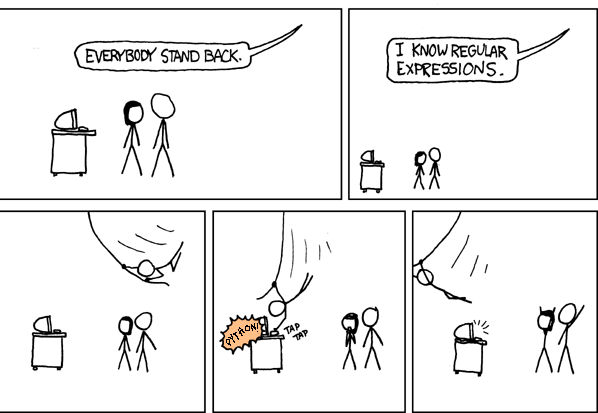
\includegraphics[scale=0.4]{images/regular_expressions_altered.png} 
\end{center}

Slightly mangled https://xkcd.com/208/

\end{frame}


\begin{frame}{Further resources}

\begin{itemize}
 \item Ask me a question now! \bigskip

 \item The Python docs are great. \lstinline$http://docs.python.org/2/library/re.html$
 \item Online tool for testing regexes: \lstinline$http://www.pythonregex.com/$
 \item {\it Mastering Regular Expressions} by Jeffrey Friedel
 \item Learn Regex the Hard Way \lstinline$http://regex.learncodethehardway.org/book/$
\end{itemize}

\end{frame}

\end{document}